\section{Prinzip}

Die Navigation unseres Modellfahrzeugs im Straßenverkehrsszenario basiert auf einer Weltkarte, in der alle bereits erkannten Punkte, die zu einer Fahrbahnmarkierung gehören, eingetragen werden. Zu Anfang wurde im Kapitel~\ref{sec:ks} beschrieben, dass das Roboterkoordinatensystem \gls{lat:RoboterKOS} die Pose des Autos darstellt. Die Pose ist der Zustandsvektor \gls{lat:statevector} aus Position \( (\gls{x},\gls{y}) \) und Orientierung \gls{gre:orientierung}.

% Formel für Pose (Zustandsvektor)
\begin{equation}
\gls{lat:statevector} = 
\begin{pmatrix}
\gls{x}(\gls{lat:time}) 	\\
\gls{y}(\gls{lat:time})	\\
\gls{gre:orientierung}(\gls{lat:time})    	\\
\end{pmatrix}
\end{equation} 

 Aus den Informationen der Weltkarte und dem aktuellen Standort des Roboters ist es möglich, eine Trajektorie zu planen, um das Fahrzeug in der Fahrspur zu halten. Daher ist es wichtig, den Zustandsvektor für jeden Regelschritt neu zu bestimmen. Zur Berechnung der neuen Position stehen uns die Wegmessungen \(s\) des Encoders und der Zeitunterschied \(\gls{lat:time}-{\gls{lat:time}}_0\) in Bezug auf die alte Pose zur Verfügung, woraus die Geschwindigkeit \gls{lat:velocity} ermittelt wird. Die Orientierung wird von der eingebauten \gls{acr:imu} gemessen und direkt in die neue Pose eingetragen. Somit ist unser Eingangsvektor \gls{lat:inputvector}
 
 % Formel für Eingangsvektor
\begin{equation}
\gls{lat:inputvector} = 
\begin{pmatrix}
\gls{lat:velocity}(\gls{lat:time}) 			\\
\gls{gre:orientierung}(\gls{lat:time})    	\\
\end{pmatrix}
, \qquad \text{mit }
\gls{lat:velocity}(\gls{lat:time}) = \frac{s}{\gls{lat:time}-{\gls{lat:time}}_0}
\end{equation} 
 
Das Besondere an einer Ackermann-Lenkung ist, dass in einer Kurvenfahrt das innen liegende Vorderrad stärker einlenkt als das Äußere, sodass sich ein gemeinsamer Schnittpunkt mit allen vier Radachsen ergibt (siehe Abb.~\ref{fig:regelung_prinzip_modell}). Dieser Punkt wird auch als \gls{acr:icr} bezeichnet und beschreibt den Mittelpunkt der gefahrenen Kreisbahn. 

% Bild Ackermann-Lenkung
\begin{figure}[H] % [htb]
  \centering
  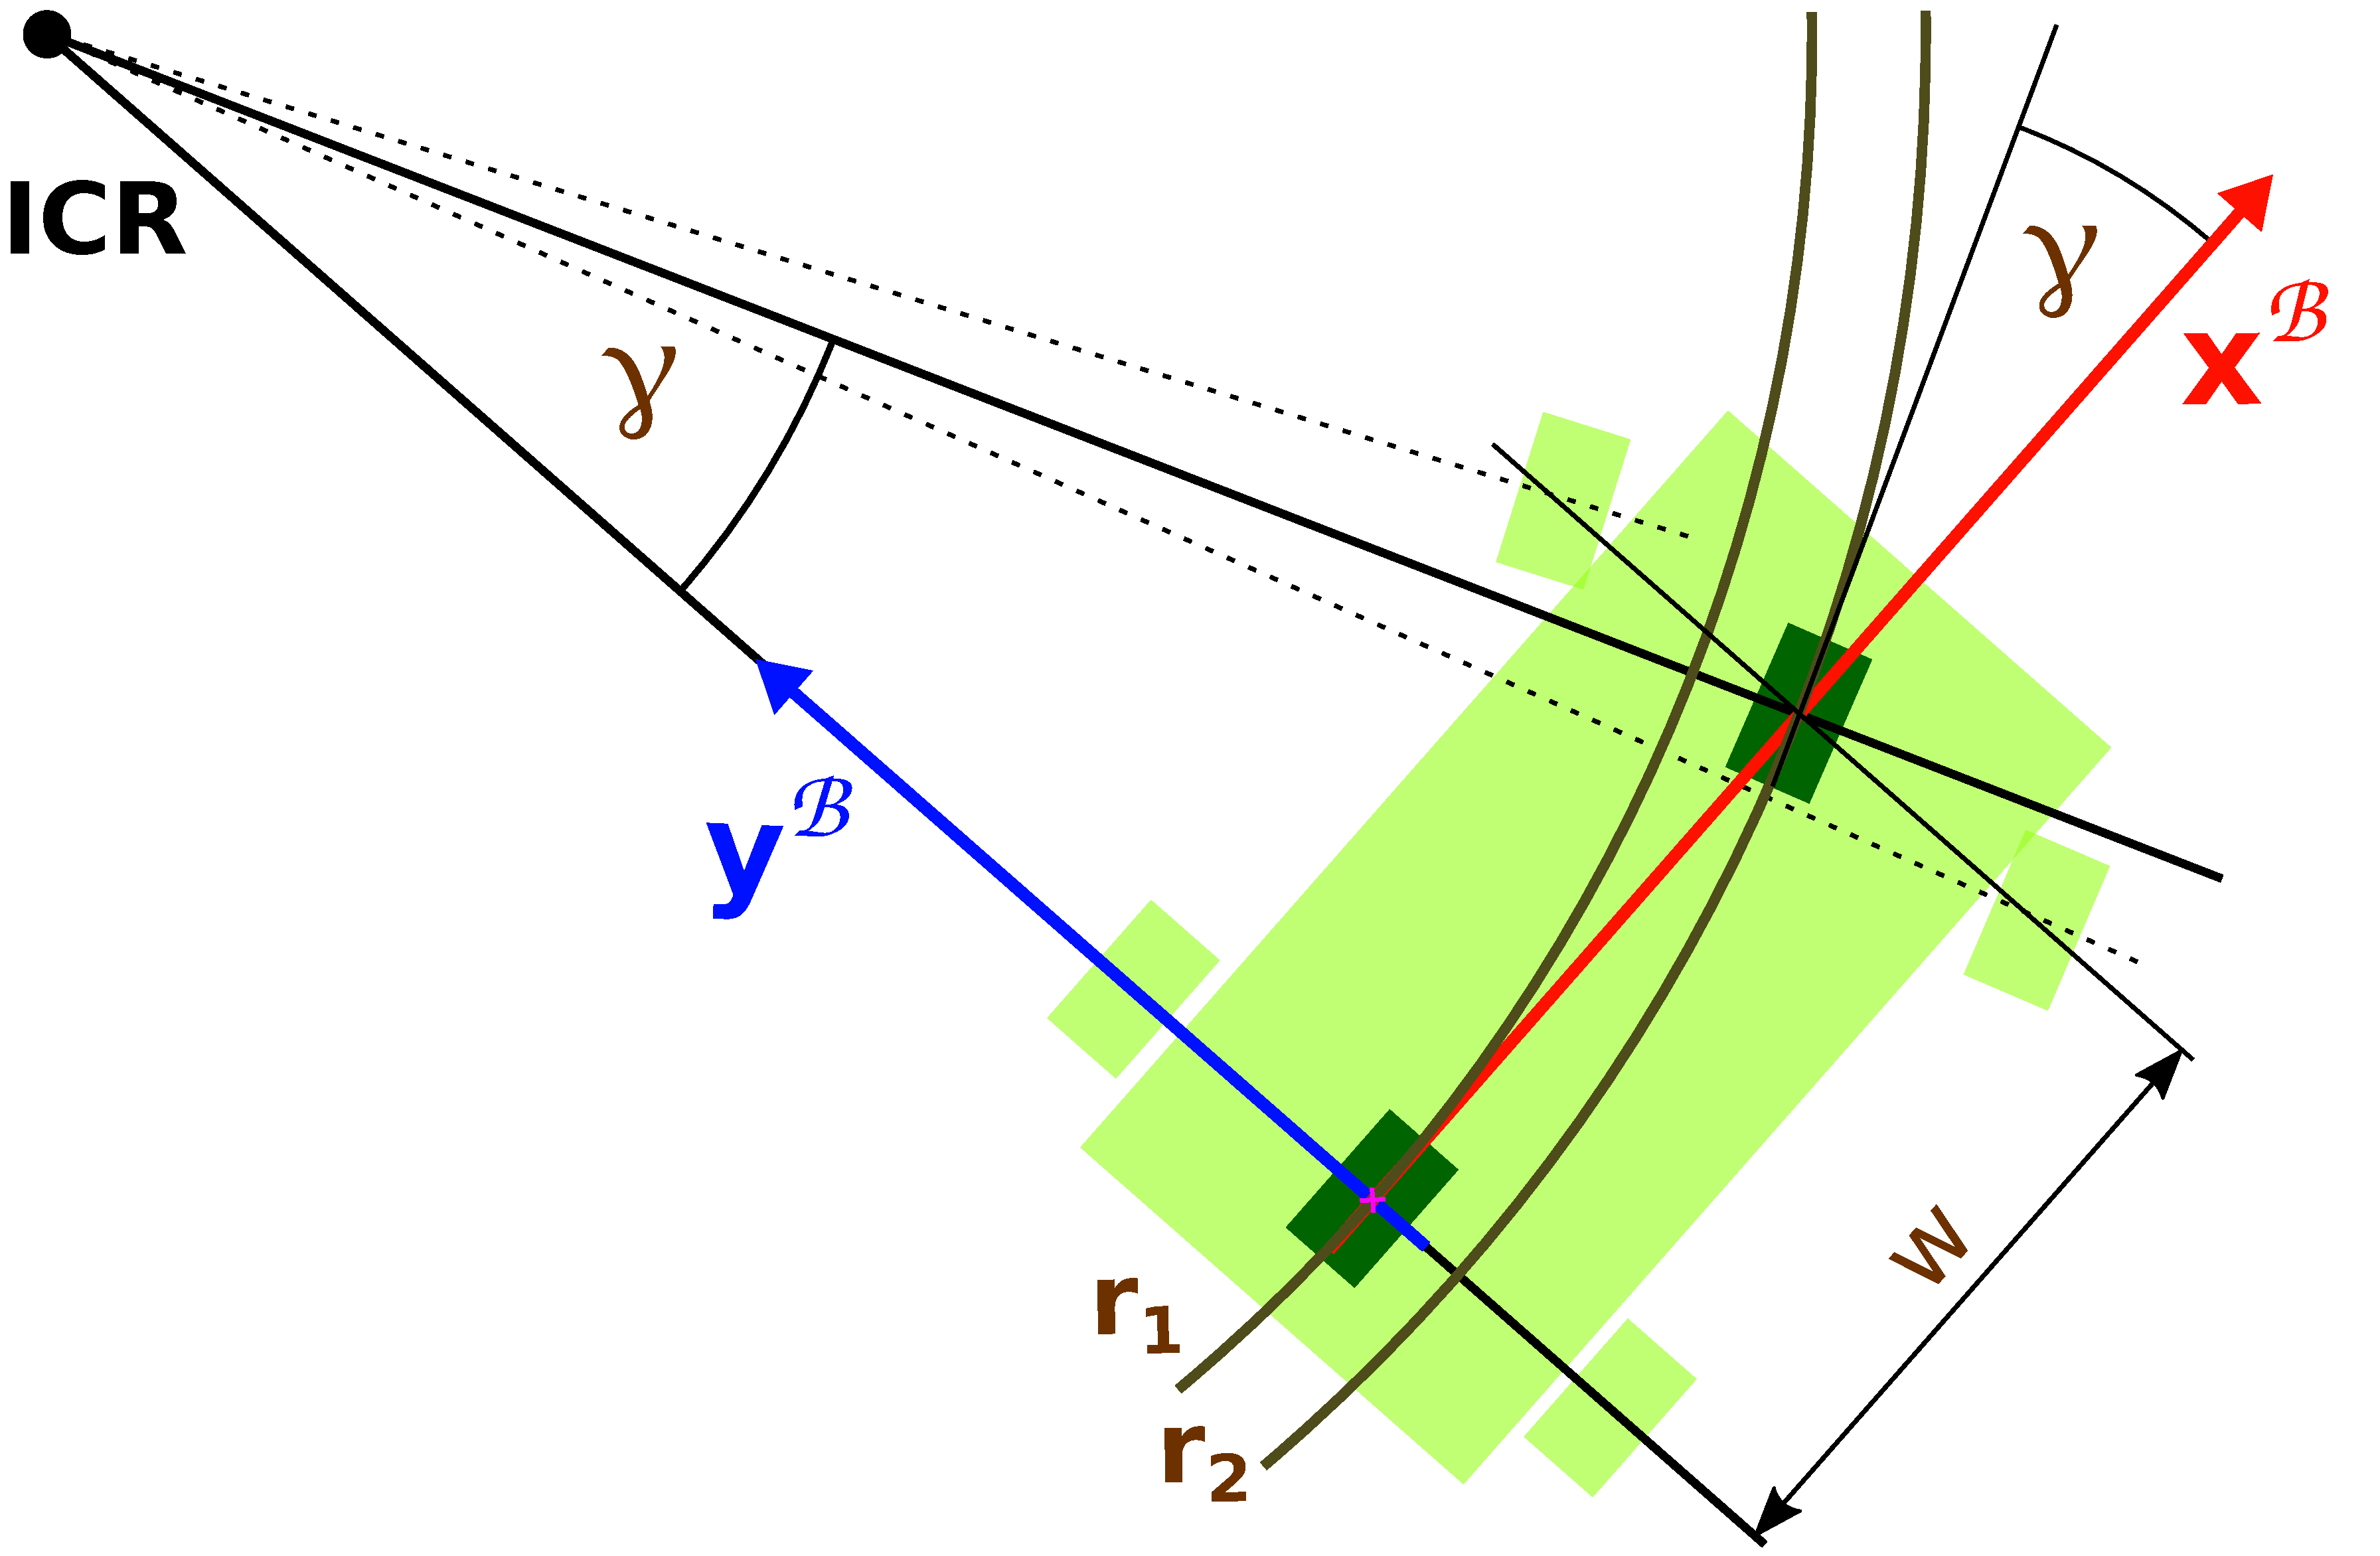
\includegraphics[width=0.9\textwidth]{regelung_prinzip_modell.pdf}
  \caption{Modellierung der Ackermannlenkung durch übliche Vereinfachung auf das Bicycle-Modell}
  \label{fig:regelung_prinzip_modell}
\end{figure}

Zur leichteren mathematischen Beschreibung des Fahrzeugs mit Ackermannlenkung wird das Modell üblicherweise auf das eines Zweirades reduziert (\emph{Bicycle-Modell}). Der Kreisradius ist dann der Abstand vom \gls{acr:icr} zum Ursprung des Roboterkoordinatensystems. Außerdem lässt sich \gls{gre:lenkwinkel} wie in Abbildung~\ref{fig:regelung_prinzip_modell} gezeigt im Winkel der beiden Radachsen zueinander wiederfinden. Nachfolgende Formel~\ref{eq:regelung_prinzip_fahrzeugmodell} zum vereinfachten Fahrzeugmodell in Weltkoordinaten \gls{lat:WeltKOS} ist aus \autocite{corkeRoboticsVisionControl2017} entnommen. Unser Eingangsvektor besteht neben der Geschwindigkeit \gls{lat:velocity}(\gls{lat:time}) allerdings nicht aus dem Lenkwinkel \gls{gre:lenkwinkel}, sondern aus der Orientierung \gls{gre:orientierung}, weshalb bei uns die Berechnung von \gls{gre:orientierung} aus \gls{gre:lenkwinkel} nicht zum Einsatz kommt. 

% Formel Fahrzeugmodell
\begin{equation}
\dot{\gls{lat:statevector}} = 
\begin{pmatrix}
\dot{\gls{x}}(\gls{lat:time}) 	\\
\dot{\gls{y}}(\gls{lat:time})	\\
\dot{\gls{gre:orientierung}}(\gls{lat:time})    	\\
\end{pmatrix}
=
\begin{pmatrix}
\gls{lat:velocity} \cdot \cos \gls{gre:orientierung} 	\\
\gls{lat:velocity} \cdot \sin \gls{gre:orientierung} 	\\
\frac{\gls{lat:velocity}}{\gls{lat:radstand}} \cdot \tan \gls{gre:lenkwinkel}    	\\
\end{pmatrix}
\label{eq:regelung_prinzip_fahrzeugmodell}
\end{equation} 

Das Modellfahrzeug wird nach dem \glqq Pure-Pursuit\grqq-Regler gesteuert. In einem bestimmten Abstand vor dem Auto wird ein Zielpunkt gesetzt, zu welchem bis zur Erstellung eines neuen Zielpunktes navigiert werden soll. Da wir den Schlupf der Räder vernachlässigt haben, ist das Erreichen des Zielpunktes völlig unabhängig von der Geschwindigkeit und nur noch an den Lenkwinkel gebunden. Dieser wird so eingestellt, dass die sich dadurch einstellende Kreisbahn durch den Zielpunkt verläuft. Wie der Zielpunkt und der dazu passende Lenkwinkel \gls{gre:lenkwinkel} ermittelt werden, beschreiben die nun folgenden zwei Abschnitte.
